
\documentclass[10pt]{article}
\usepackage[spanish]{babel}
\selectlanguage{spanish}
\usepackage[utf8]{inputenc}
\usepackage{graphicx}
\usepackage[lmargin=3cm,rmargin=3cm,tmargin=3cm,bmargin=3cm]{geometry}
\usepackage{amsmath}
\usepackage{amsfonts}
\usepackage{amssymb}
\title{Usando Gnuplot}
\author{Luisa Fernanda Orci Fernandez.}
\date{28 de Febrero del 2015}


\begin{document}

\maketitle
\section{Teorema de Taylor}
El teorema de Taylor, o mejor conocido como el polinomio de Taylor, nos permite obtener aproximaciones polinómicas de una función, también permite calcular el error obtenido mediante esta estimación.\\
Este teorema recibe su nombre del matematico Brook Taylor, ya que el lo enunció con mas generalidad en 1712, a pesar de que fue descubierto por James Gregory en 1671.\\

El polinomio de taylor: 
$$f(x) = f(x_0)+f'(x_0)(x-x_0)+{{f^{(2)}(x_0)}\over{2!}}{{(x-x_0)^2}}+{{f^{(3)}(x_0)}\over{3!}}{{(x-x_0)^3}}+\cdots +{{f^{(n)}(x_0)}\over{n!}}{{(x-x_0)^n}} + E_{n} $$

Calcular el error:
$$ E_n = {{f^{(n+1)}(c)}\over{(n+1)!}}{{(x-x_0)^{(n+1)}}} $$

La forma reducida: 
$$ f(x) = \sum_{k=0}^n {{f^{(k)}(x_0)}\over{k!}}{{(x-x_0)^{k}}} + E_n$$

\section{Aproximaciones}
Esta actividad consiste en realizar algunas aproximaciones de grado n utilizando el teorema de Taylor, para ello utilizaremos el programa en línea wxMaxima.

\newpage

\subsection{Aproximación para $sin(x)$}
\subsection*{Código:}
\begin{verbatim}
f(x):=sin(x);
P1(x):=taylor(f(x), x, 0, 1);
P3(x):=taylor(f(x), x, 0, 3);
P5(x):=taylor(f(x), x, 0, 5);
P7(x):=taylor(f(x), x, 0, 7);
tex(P1(x));
tex(P3(x));
tex(P5(x));
tex(P7(x));
plot2d ([P1(x), P3(x), P5(x), P7(x), f(x)], [x, -%pi, %pi],
[color, blue, green, red, black, cyan], [legend, "f", "P1", "P3", "P5", "P7"],[axes, true], [xlabel, "x"], 
[ylabel, "sin(x)"]);
\end{verbatim}

\subsection*{Resultados:}
\begin{enumerate}
\item P1 = $+x+\cdots $
\item P3 = $x-{{x^3}\over{6}}+\cdots $
\item P5 = $x-{{x^3}\over{6}}+{{x^5}\over{120}}+\cdots $
\item P7 = $x-{{x^3}\over{6}}+{{x^5}\over{120}}-{{x^7}\over{5040}}+\cdots $
\end{enumerate}
\subsection*{Gráfica:} 
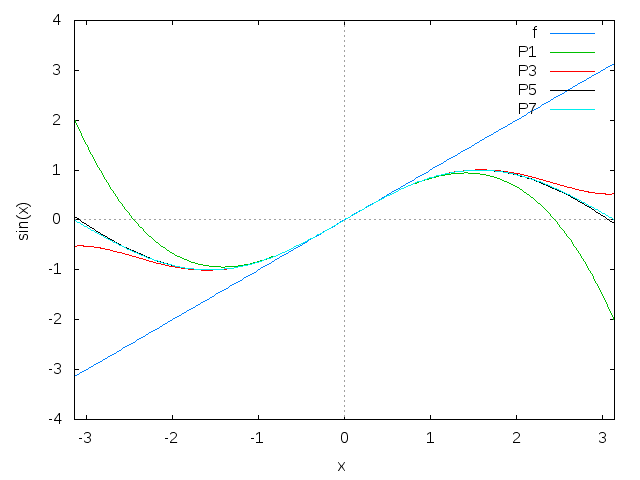
\includegraphics[scale=0.6]{plot}

\newpage
\subsection{Aproximación para $log(1+x)$}
\subsection*{Código:}
\begin{verbatim}
f(x):=log(1+x);
T4(x):=taylor(f(x), x, 0, 4);
T7(x):=taylor(f(x), x, 0, 7);
T11(x):=taylor(f(x), x, 0, 11);
T16(x):=taylor(f(x), x, 0, 16);
tex(T4(x));
tex(T7(x));
tex(T11(x));
tex(T16(x));
plot2d ([T4(x), T7(x), T11(x), T16(x), f(x)], [x, -1.5, 1.5], [y, -4,2],[color, red, green, blue, cyan, orange],
[legend, "T4", "T7", "T11", "T16", "f"],[axes, true], 
[xlabel,"x"], [ylabel, "log(1+x)"]);
\end{verbatim}

\subsection*{Resultados:}
\begin{enumerate}
\item T4 = $x-{{x^2}\over{2}}+{{x^3}\over{3}}-{{x^4}\over{4}}+\cdots $
\item T7 = $x-{{x^2}\over{2}}+{{x^3}\over{3}}-{{x^4}\over{4}}+{{x^5}\over{5}}-
 {{x^6}\over{6}}+{{x^7}\over{7}}+\cdots $
\item T11 = $x-{{x^2}\over{2}}+{{x^3}\over{3}}-{{x^4}\over{4}}+{{x^5}\over{5}}-
 {{x^6}\over{6}}+{{x^7}\over{7}}-{{x^8}\over{8}}+{{x^9}\over{9}}-{{x
 ^{10}}\over{10}}+{{x^{11}}\over{11}}+\cdots $
\item T16 = $x-{{x^2}\over{2}}+{{x^3}\over{3}}-{{x^4}\over{4}}+{{x^5}\over{5}}-
 {{x^6}\over{6}}+{{x^7}\over{7}}-{{x^8}\over{8}}+{{x^9}\over{9}}-{{x
 ^{10}}\over{10}}+{{x^{11}}\over{11}}-{{x^{12}}\over{12}}+{{x^{13}
 }\over{13}}-{{x^{14}}\over{14}}+{{x^{15}}\over{15}}-{{x^{16}}\over{
 16}}+\cdots $
\end{enumerate}
\subsection*{Gráfica:}
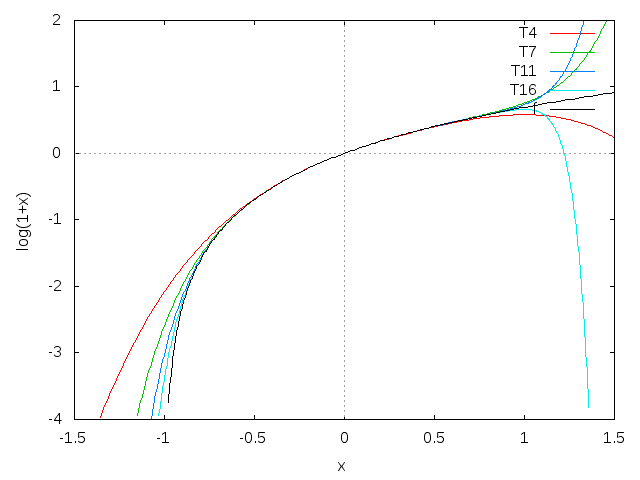
\includegraphics[scale=0.6]{plot2}

\newpage
\subsection{Aproximación para $log(cos(x))$}

\subsection*{Código:}
\begin{verbatim}
f(x):=log(cos(x));
t3(x):=taylor(f(x), x, 0, 3);
t6(x):=taylor(f(x), x, 0, 6);
t9(x):=taylor(f(x), x, 0, 9);
t12(x):=taylor(f(x), x, 0, 12);
tex(t3(x));
tex(t6(x));
tex(t9(x));	
tex(t12(x));
plot2d ([f(x), t3(x), t6(x), t9(x), t12(x)], [x, -0.5*%pi, 0.5*%pi], [y, -2,0.5],
[color, green, blue, red, cyan, orange], 
[legend, "f", "t3", "t6", "t9", "t12"], [axes, true], [xlabel,"x"], [ylabel, "log(cos(x))"]);
\end{verbatim}
\subsection*{Resultados:}
\begin{enumerate}
\item t3 = $+\left(-{{x^2}\over{2}}\right)+\cdots $
\item t6 = $-{{x^2}\over{2}}-{{x^4}\over{12}}-{{x^6}\over{45}}+\cdots $
\item t9 = $-{{x^2}\over{2}}-{{x^4}\over{12}}-{{x^6}\over{45}}-{{17\,x^8}\over{
 2520}}+\cdots $
\item t12 = $-{{x^2}\over{2}}-{{x^4}\over{12}}-{{x^6}\over{45}}-{{17\,x^8}\over{
 2520}}-{{31\,x^{10}}\over{14175}}-{{691\,x^{12}}\over{935550}}
 +\cdots $
\end{enumerate}
\subsection*{Gráfica:}
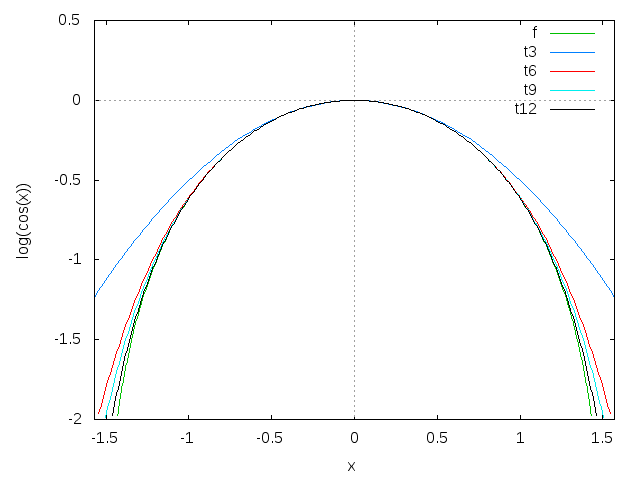
\includegraphics[scale=0.6]{plot3}

\newpage
\subsection{Aproximación para $\frac{\mathrm{e}^{x}}{cos(x)}$}
\subsection*{Código:}
\begin{verbatim}
f(x):=exp(x)/cos(x);
p4(x):=taylor(f(x), x, 0, 4);
p6(x):=taylor(f(x), x, 0, 6);
p8(x):=taylor(f(x), x, 0, 8);
p10(x):=taylor(f(x), x, 0, 10);
tex(p4(x));
tex(p6(x));
tex(p8(x));
tex(p10(x));
plot2d ([f(x), p4(x), p6(x), p8(x), p10(x)], [x, -4, 4], [y, -3,10], 
[color, blue, cyan, green, red, orange], 
[legend, "f", "p4", "p6", "p8","p10"], 
[axes, true], [xlabel,"x"], [ylabel, "exp(x)/cos(x)"]);
\end{verbatim}

\subsection*{Resultados:}
\begin{enumerate}
\item p4 = $1+x+x^2+{{2\,x^3}\over{3}}+{{x^4}\over{2}}+\cdots $
\item p6 = $1+x+x^2+{{2\,x^3}\over{3}}+{{x^4}\over{2}}+{{3\,x^5}\over{10}}+{{19
 \,x^6}\over{90}}+\cdots $
\item p8 = $1+x+x^2+{{2\,x^3}\over{3}}+{{x^4}\over{2}}+{{3\,x^5}\over{10}}+{{19
 \,x^6}\over{90}}+{{13\,x^7}\over{105}}+{{31\,x^8}\over{360}}+\cdots $
\item p10 = $1+x+x^2+{{2\,x^3}\over{3}}+{{x^4}\over{2}}+{{3\,x^5}\over{10}}+{{19
 \,x^6}\over{90}}+{{13\,x^7}\over{105}}+{{31\,x^8}\over{360}}+{{163\,
 x^9}\over{3240}}+{{3961\,x^{10}}\over{113400}}+\cdots $
\end{enumerate}
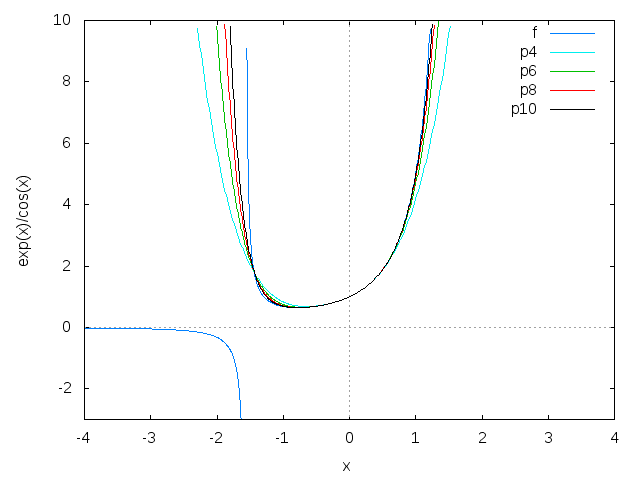
\includegraphics[scale=0.6]{plot4}

\newpage 
\subsection{Aproximación para $(1+x)(\mathrm{e}^{x})$}
\subsection*{Código:}
\begin{verbatim}
f(x):=(1+x)*exp(x);
g5(x):=taylor(f(x), x, 0, 5);
g8(x):=taylor(f(x), x, 0, 8);
g11(x):=taylor(f(x), x, 0, 11);
g14(x):=taylor(f(x), x, 0, 14);
tex(g5(x));
tex(g8(x));
tex(g11(x));
tex(g14(x));
plot2d ([g5(x), g8(x), g11(x), g14(x), f(x)], [x, -6, 2], [y, -3,6], 
[color, red, green, blue, cyan, orange], [legend, "f", "T4", "T7", "T11", "T16"], 
[axes, true], [xlabel,"x"], [ylabel, "(1+x)*exp(x)"]);
\end{verbatim}
\subsection*{Resultados:}
\begin{enumerate}
\item g5 = $1+2\,x+{{3\,x^2}\over{2}}+{{2\,x^3}\over{3}}+{{5\,x^4}\over{24}}+{{
 x^5}\over{20}}+\cdots $
\item g8 = $1+2\,x+{{3\,x^2}\over{2}}+{{2\,x^3}\over{3}}+{{5\,x^4}\over{24}}+{{
 x^5}\over{20}}+{{7\,x^6}\over{720}}+{{x^7}\over{630}}+{{x^8}\over{
 4480}}+\cdots $
\item g11 = $1+2\,x+{{3\,x^2}\over{2}}+{{2\,x^3}\over{3}}+{{5\,x^4}\over{24}}+{{
 x^5}\over{20}}+{{7\,x^6}\over{720}}+{{x^7}\over{630}}+{{x^8}\over{
 4480}}+{{x^9}\over{36288}}+{{11\,x^{10}}\over{3628800}}+{{x^{11}
 }\over{3326400}}+\cdots $
\item g14 = $1+2\,x+{{3\,x^2}\over{2}}+{{2\,x^3}\over{3}}+{{5\,x^4}\over{24}}+{{
 x^5}\over{20}}+{{7\,x^6}\over{720}}+{{x^7}\over{630}}+{{x^8}\over{
 4480}}+{{x^9}\over{36288}}+{{11\,x^{10}}\over{3628800}}+{{x^{11}
 }\over{3326400}}+{{13\,x^{12}}\over{479001600}}+{{x^{13}}\over{
 444787200}}+{{x^{14}}\over{5811886080}}+\cdots $
\end{enumerate}
\subsection*{Gráfica:}
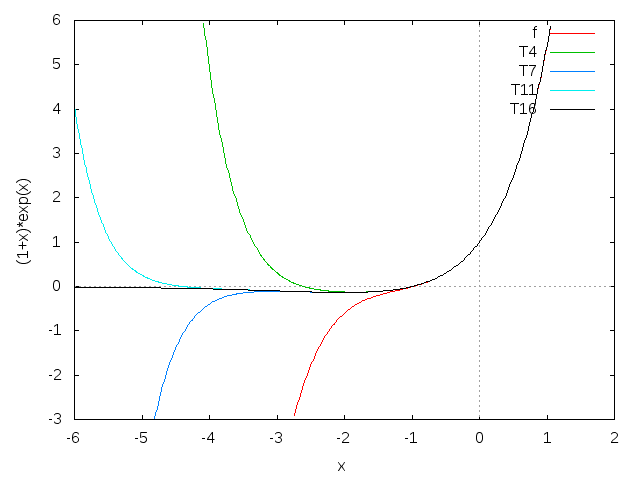
\includegraphics[scale=0.6]{plot5}

\end{document}